\documentclass{beamer}
\usetheme{Madrid} % My favorite!
%\usetheme{Boadilla} % Pretty neat, soft color.
%\usetheme{default}
%\usetheme{Warsaw}
%\usetheme{Bergen} % This template has nagivation on the left
%\usetheme{Frankfurt} % Similar to the default 
%with an extra region at the top.
%\usecolortheme{seahorse} % Simple and clean template
%\usetheme{Darmstadt} % not so good
% Uncomment the following line if you want %
% page numbers and using Warsaw theme%
% \setbeamertemplate{footline}[page number]
%\setbeamercovered{transparent}
\setbeamercovered{invisible}
% To remove the navigation symbols from 
% the bottom of slides%
\setbeamertemplate{navigation symbols}{} 
%
\usepackage{graphicx}
%\usepackage{bm}         % For typesetting bold math (not \mathbold)
%\logo{\includegraphics[height=0.6cm]{yourlogo.eps}}

\graphicspath{{./extra/}}

%
\title[Graphical models of obesity]{A set of graphical models to explore the effects of globalization and development on the prevalence of obesity}
\author{Shannon Cebron, Zhendan Zhu, Michael Weinberger}
\institute[Johns Hopkins University]
{
Johns Hopkins University \\
\medskip
{\emph{scebron@cis.jhu.edu, zzhu11@johnshopkins.edu, michael.lee.weinberger@gmail.com}}
}
\date{\today}
% \today will show current date. 
% Alternatively, you can specify a date.
%
\begin{document}
%
\begin{frame}
\titlepage
\end{frame}
%
\begin{frame}
\frametitle{Summary}
\begin{block}
{Project overview}
-Under-explored phenomenon
\\
-Graphical models to represent global connections
\\
-Statistical models to analyze graphical features
\end{block}
\end{frame}
%
\begin{frame}
\frametitle{Sponsor}
\begin{block}
{The RAND Corporation}
-Nonpartisan public policy research organization
\\
-A focus area is health and health care
\\
-Has previously worked with the US Congress
\end{block}
\end{frame}
%

\begin{frame}
\frametitle{Background}
\begin{block}
{What is obesity?}
-Defined as a BMI greater than 30 (kilograms of body weight per meters of height squared)
\\
-Indicator for heart disease, diabetes, and more
\\
-Causes bone density and joint problems and difficulty with everyday tasks
\end{block}
\end{frame}

\begin{frame}
\frametitle{Background}
\begin{block}
{Costs to society}
-Leading cause of preventable death
\\
-Drives up health care costs
\\
-Lost hours affect the economy (117 billion USD per year in the USA)
\end{block}
\end{frame}

\begin{frame}
\frametitle{Background}
\begin{block}
{Relationship to globalization}
-Increasing at highest rates in developed countries
\\
-Increasing at higher rates in neighbors of developed countries
\\
-Burger King in Accra, Ghana
\\
-Exploding urbanization in places like Burundi
\end{block}
\end{frame}

\begin{frame}
\frametitle{Deliverables}
\begin{block}
{Regression model}
-A model to predict current obesity rate based on known data
\end{block}
\end{frame}

\begin{frame}
\frametitle{Deliverables}
\begin{block}
{Interactive experience}
-An R package to encapsulate obesity prediction models
\\
-Allows user manipulation of data to predict effects of policy changes
\\
-Includes sample data
\end{block}
\end{frame}
 
\begin{frame}
\frametitle{Project outline}
\begin{block}
{Data acquisition}
-Obesity rate
\\
-Development status
\\
-Bordering nations
\\
-Economic data
\\
-Trading data
\\
{\emph{Source: CIA World Factbook}}
\end{block}
\end{frame}

\begin{frame}
\frametitle{Project outline}
\begin{block}
{Graph construction}
-Nations as vertices
\\
-Varying adjacency and edge length definitions for each graph
\\
-Example: Border relationships as adjacencies and distance between capital cities as edge lengths
\\
{\emph{Environment: Python}}
\end{block}
\end{frame}

\begin{frame}
\frametitle{Project outline}
\begin{block}
{Data extraction}
-Neighborhood sizes
\\
-Shortest path to a developed country
\end{block}
\end{frame}

\begin{frame}
\frametitle{Project outline}
\begin{block}
{Data analysis}
{\emph {Independent variables (examples)}}
\begin{itemize}
\item GDP per capita
\item Education expenditures as a percentage of GDP
\item Total internet users
\item Number of food import partners
\item Degree of separation from a highly developed nation
\item Rate of urbanization
\end{itemize}

{\emph {Dependent variable:}} Obesity rate
\end{block}
\end{frame}

\begin{frame}
\frametitle{Project outline}
\begin{block}
{Data analysis}
-R has great capability for regression diagnostics
\\
-Will consider not only linear, but also exponential, polynomial, and other regressions
\\
-An acceptable model will have a significant F-statistic and significant T-tests for slope coefficients
\\
-Model must also meet assumptions of regression
\end{block}
\end{frame}

\begin{frame}
\frametitle{Preliminary work: data analysis}
\begin{figure}
\label{fig:dataframe}
\caption{Visualization of these data in RStudio}
\centering
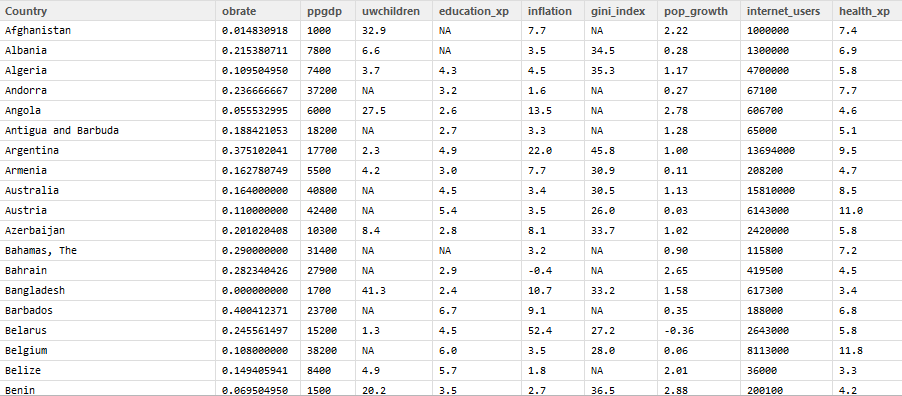
\includegraphics{dataframe_R.PNG}
\end{figure}
%use dataframe_R.PNG
\end{frame}

\begin{frame}
\frametitle{Preliminary work: data analysis}
\begin{figure}
\label{fig:simreg}
\caption{Simple regression of obesity rate on education expenditures}
\centering
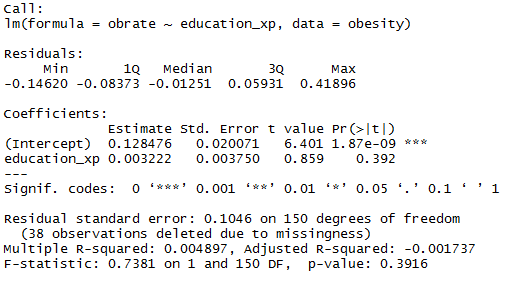
\includegraphics{edu_regression.PNG}
\end{figure}
\end{frame}

\begin{frame}
\frametitle{Preliminary work: data analysis}
\begin{figure}
\label{fig:edu_xp}
\caption{Plot of obesity rate against education expenditures, overlaid with regression line}
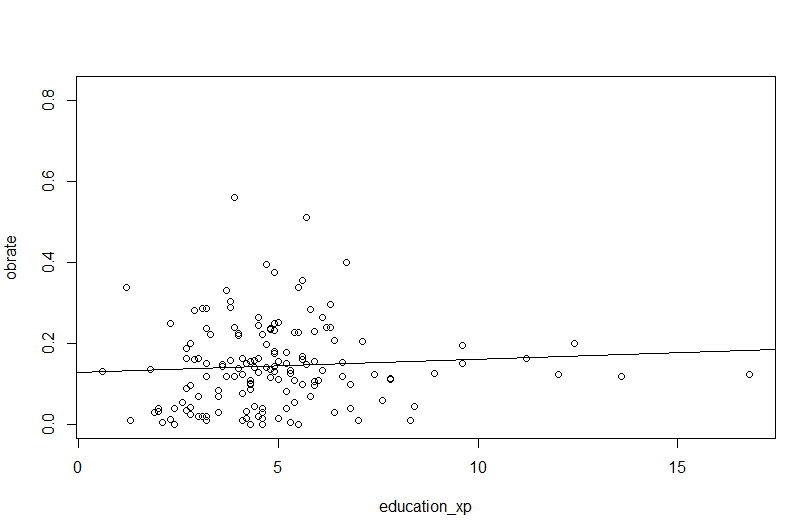
\includegraphics[scale=0.6]{edu_plot.PNG}
\end{figure}
\end{frame}

\begin{frame}
\frametitle{Preliminary work: data analysis}
\begin{figure}
\label{fig:multireg}
\caption{Multiple linear regression of obesity rate against basic independent variables}
\centering
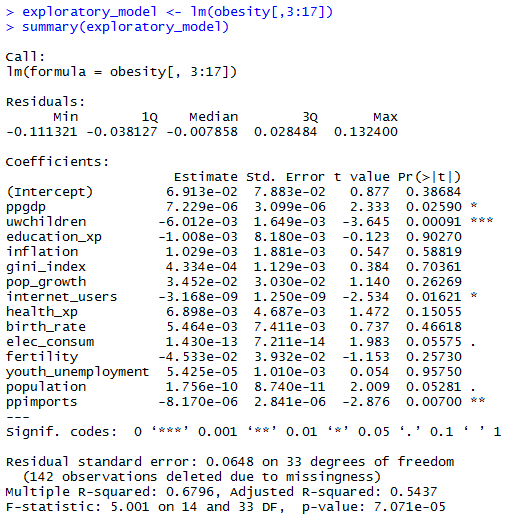
\includegraphics[scale=0.9]{multi_regression.PNG}
\end{figure}
\end{frame}

\begin{frame}
\frametitle{Preliminary work: data analysis}
\begin{figure}
\label{fig:scatter}
\caption{Scatterplox matrix of several relationships}
\centering
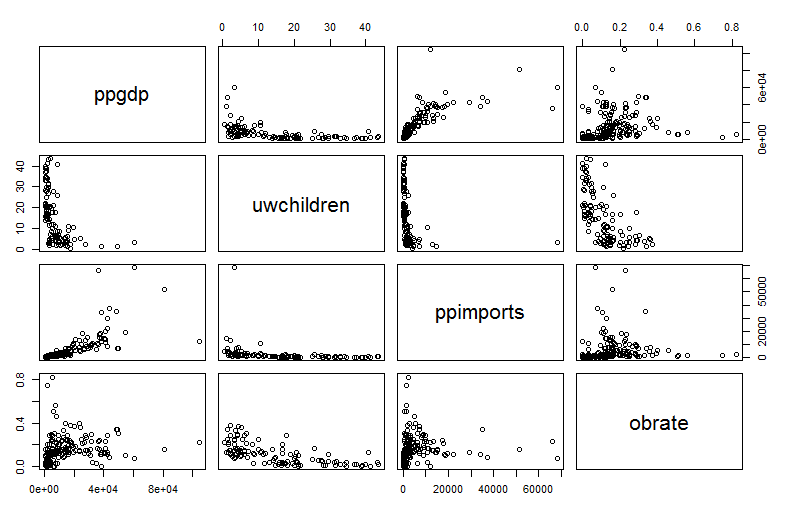
\includegraphics[scale=0.65]{scatter_matrix.PNG}
\end{figure}
\end{frame}

\begin{frame}
\frametitle{Preliminary work: data analysis}
\begin{block}
{Discovering nonlinear relationships}
-Per person imports has a weak linear relationship with obesity rate (p=0.269)
\\
-Log per person imports has a strong linear relationship with obesity rate (p=0.00000027)
\end{block}

\begin{figure}
\label{fig:logs}
\caption{Log(imports) takes on a stronger relationship with the data}
\centering
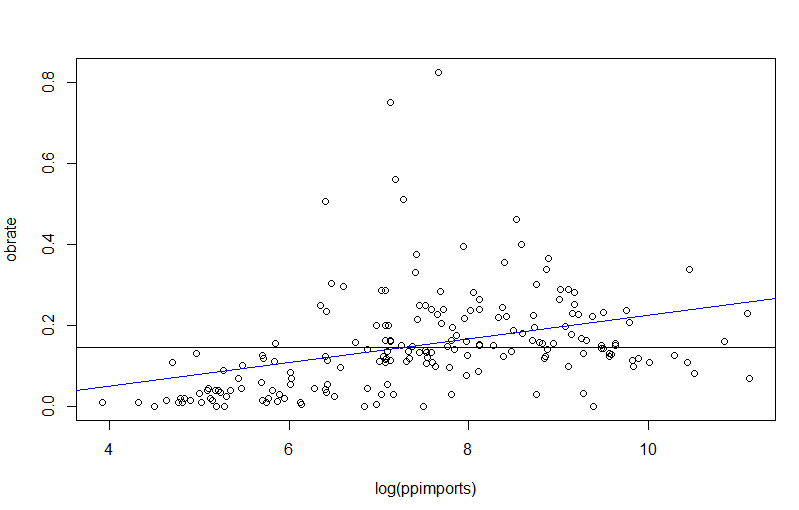
\includegraphics[scale=0.4]{ppimports_log.PNG}
\end{figure}
%blue line is better regression fit using log imports
\end{frame}

\begin{frame}
\frametitle{Preliminary work: graph construction}
\begin{figure}
\label{fig:borders}
\caption{Country border distances}
\centering
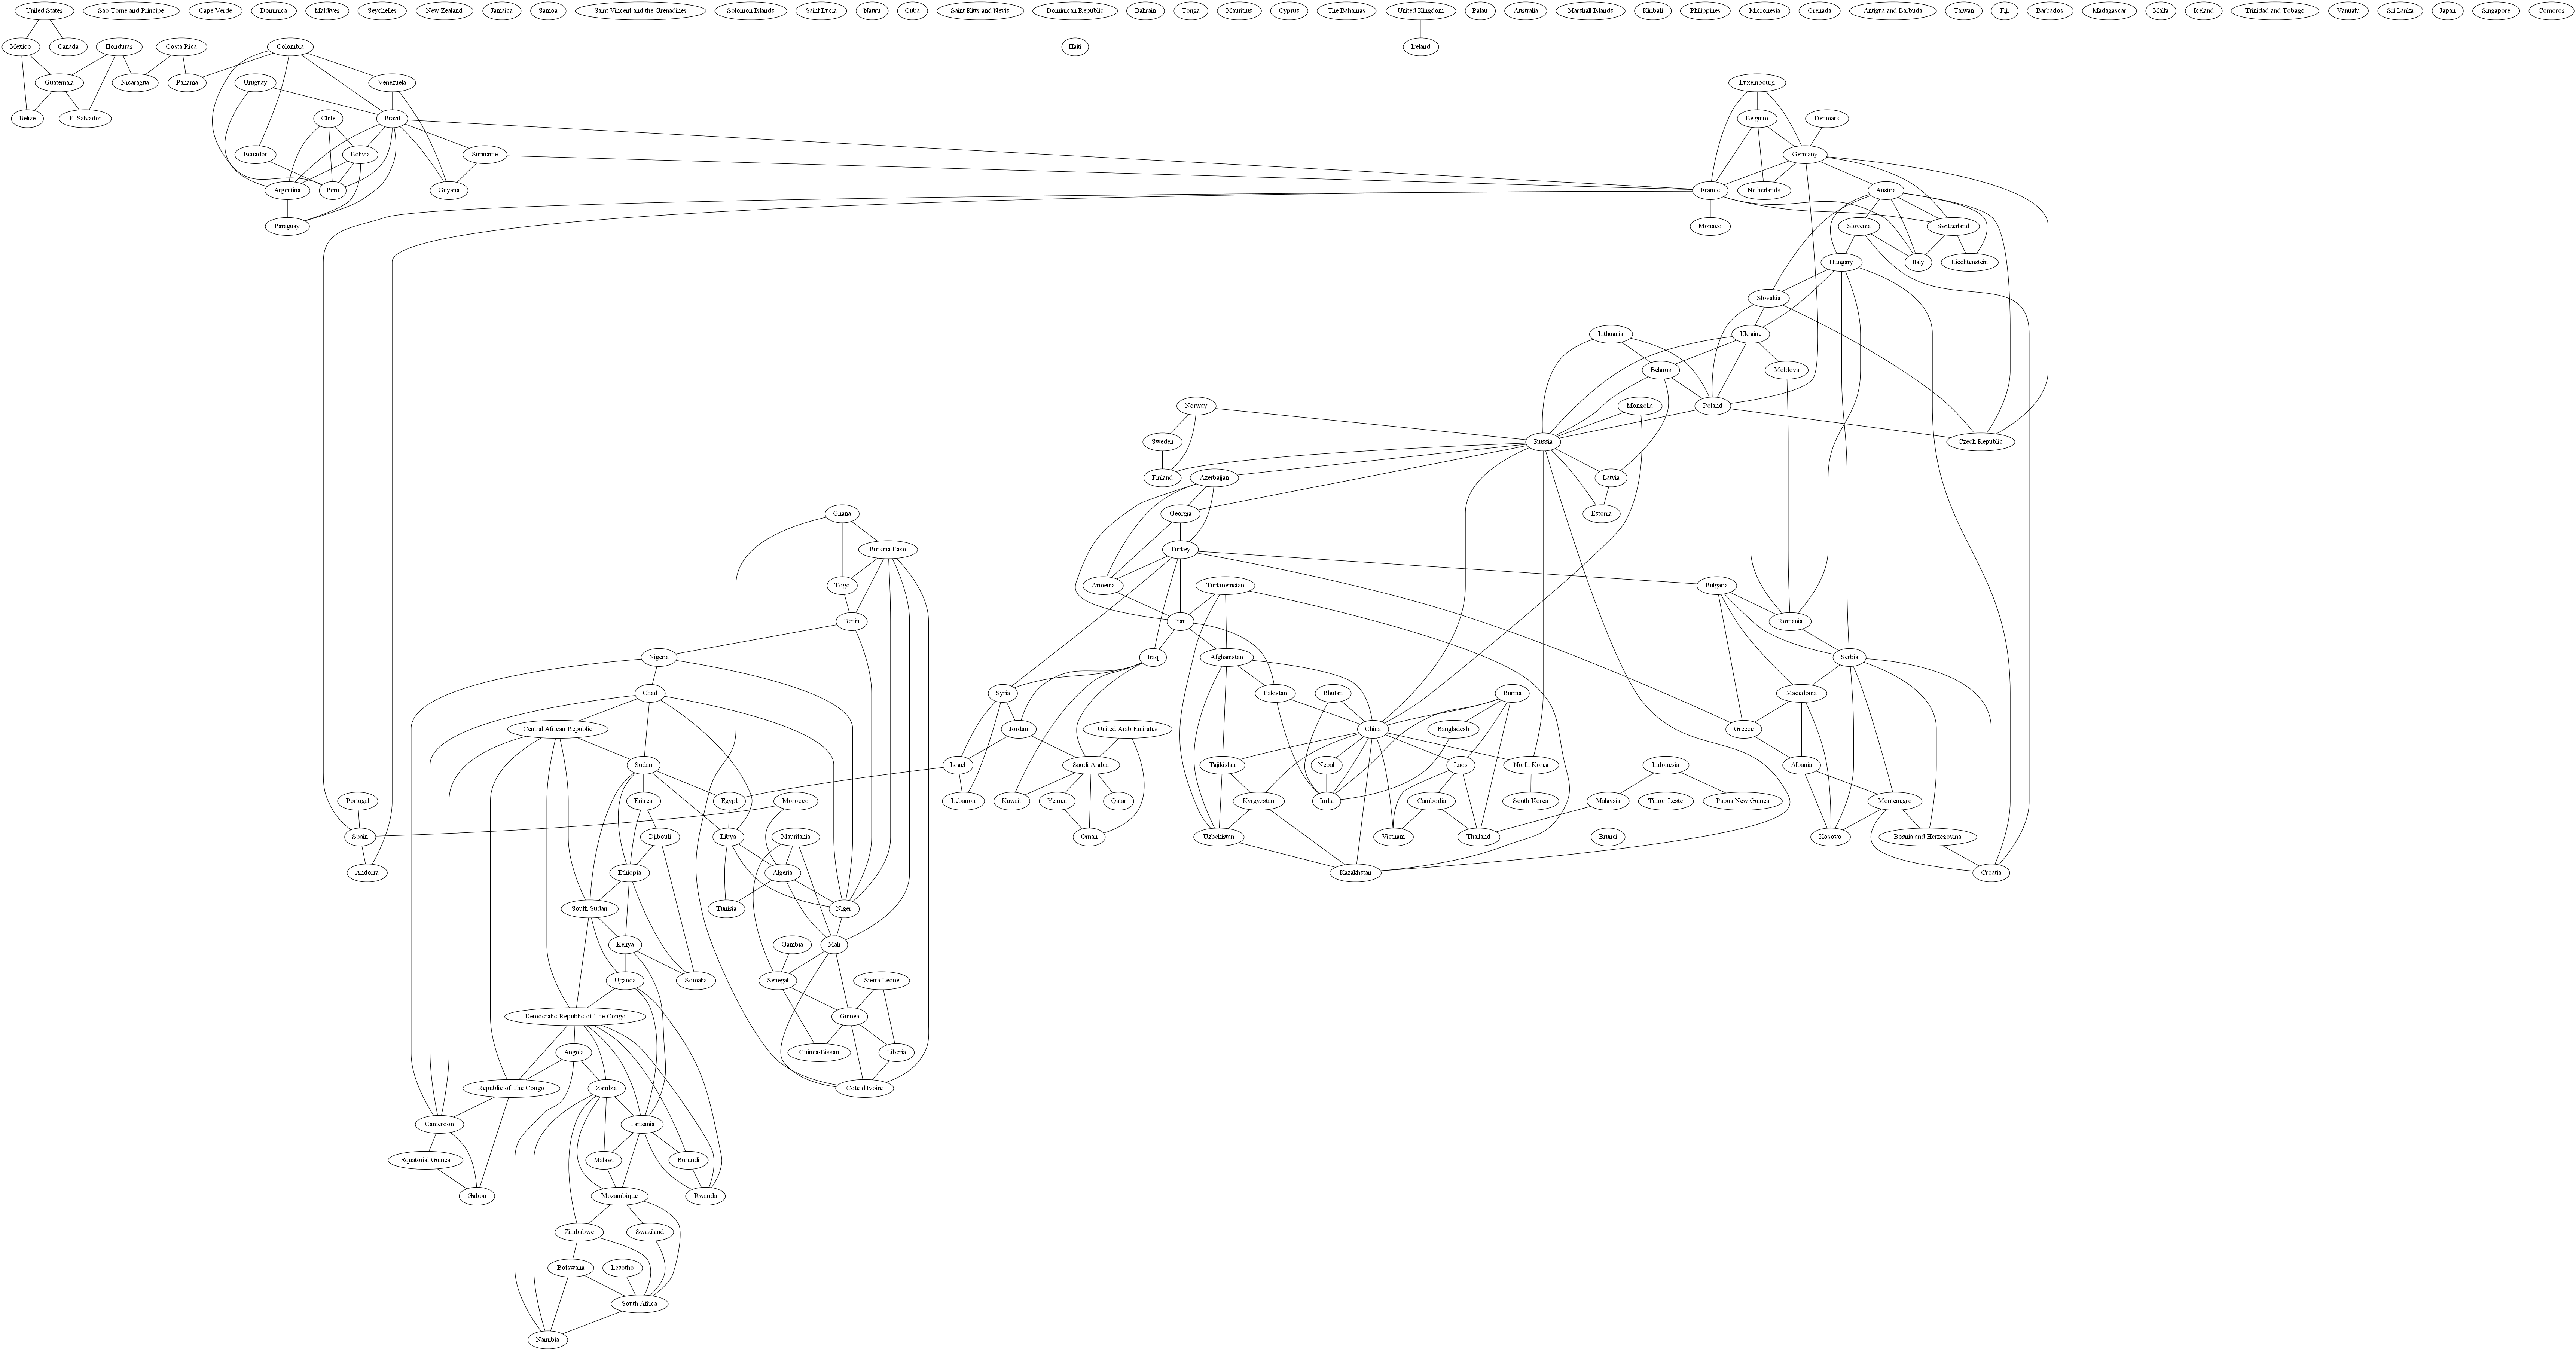
\includegraphics[scale=0.05]{edges.PNG}
\end{figure}
\end{frame}

\begin{frame}
\frametitle{Conclusion}
\begin{block}
{Remaining work to be done}
-Extracting data from graphs and importing into R
\\
-Regression analysis using this new data
\\
-Creation of deliverables
\end{block}

\begin{block}
{Looking forward}
-Future research might including a more in-depth exploration of graphical variables
\\
-Efforts may be taken to find obesity data for more than 190 countries
\\
-More lifestyle data and cultural factors could be considered, such as popularity of sports
\end{block}
\end{frame}
 

\begin{frame}[fragile]
    \frametitle{Q and A}
\begin{itemize}
            \visible<1,2>{\item Question: Is the United States the most obese country? If not, which country is?}
            \visible<2>{\item Answer: Nauru and Micronesia, two Polynesian island nations, are the most obese and second most obese countries.}
\end{itemize}
\end{frame}

\begin{frame}[fragile]
    \frametitle{Q and A}
\begin{itemize}
            \visible<1,2>{\item Question: Are there any two obesity predictors that might be telling us the same thing? How did you account for this?}
            \visible<2>{\item Answer: Yes. We have avoided this prediction conflict by choosing between the variables or by somehow merging them.}
\end{itemize}
\end{frame}

\begin{frame}
\centerline{The End}
\end{frame}
% End of slides
\end{document} 